% simianer-regexvis.tex
% Patrick Simianer <p@simianer.de>
% YYYY-MM-DD
\documentclass[ignorenonframetext]{beamer}

\mode<presentation>
{
  \usetheme{Singapore}
  \usecolortheme{dolphin}
  \usefonttheme{professionalfonts}
  \useinnertheme{circles}
  \useoutertheme{miniframes}
  \setbeamertemplate{navigation symbols}{}
  \beamersetuncovermixins{\opaqueness<1>{5}}{\opaqueness<2->{15}}
  \setbeamertemplate{footline}[frame number]
}

\usepackage[utf8]{inputenc}
\usepackage[T1]{fontenc}
\usepackage[ngerman]{babel}
\usepackage{lmodern}
\usepackage{framed}
\usepackage{color}


\title[regexvis]{Patrick Simianer\\ Visualisierung Regulärer Ausdrücke}
\author{Patrick~Simianer \tiny 2508483\\\normalsize 2010-06-28}
\date{Endliche Automaten HS bei Dr. Karin Haenelt\\ Universitiät Heidelberg im Sommersemester 2010}

\AtBeginSection[]{%
\begin{frame}
\tableofcontents[currentsection]
\end{frame}
}% AtBeginSection



\begin{document}



%%%%%%%%%%%%%%%%%%%%%%%%%%%%%%%%%%%%%%%%%%%%%%%%%%%%%%%%%%%%%%%%%%%%%%%%%%%%%%
\frame[plain]{\titlepage}
%%%%%%%%%%%%%%%%%%%%%%%%%%%%%%%%%%%%%%%%%%%%%%%%%%%%%%%%%%%%%%%%%%%%%%%%%%%%%%



%%%%%%%%%%%%%%%%%%%%%%%%%%%%%%%%%%%%%%%%%%%%%%%%%%%%%%%%%%%%%%%%%%%%%%%%%%%%%%
\begin{frame}[plain]
    \frametitle{Gliederung}
    \tableofcontents
\end{frame}
%%%%%%%%%%%%%%%%%%%%%%%%%%%%%%%%%%%%%%%%%%%%%%%%%%%%%%%%%%%%%%%%%%%%%%%%%%%%%%



%%%%%%%%%%%%%%%%%%%%%%%%%%%%%%%%%%%%%%%%%%%%%%%%%%%%%%%%%%%%%%%%%%%%%%%%%%%%%%
\section{Vorhaben}


\begin{frame}
    \frametitle{Vorhaben}
	
	\begin{itemize}
		\item[] \textbf{Darstellung der Funktionsweise regulärer Ausdrücke}
		\item[]
		\item[$\Rightarrow$] Eigene Implementierung
	\end{itemize}
\end{frame}

\begin{frame}
    \frametitle{asdf}

	\begin{itemize}
		\item Mögliche Implementierungen
		\begin{enumerate}
			\item Backtracking
			\item Endliche Automaten
		\end{enumerate}
	\end{itemize}
\end{frame}

\begin{frame}
    \frametitle{Notwendige Schritte/Umsetzung}
	
	\begin{enumerate}
		\item \textbf{Parsen} des Ausdrucks
		\item Umsetzung in einen \textbf{nichtdeterministischen endlichen Automaten}
		\item Übersetzung in einen \textbf{deterministischen} endlichen Automaten
		\item Graphische \textbf{Darstellung} des Automaten und dessen \textbf{Simulation}
		\item[]
		\item[$\Rightarrow$] Umsetzung im \textbf{Browser}: \textit{JavaScript} (\textit{jQuery}, \textit{Rapha\"elJS}) , \textit{HTML}, \textit{CSS}, \textit{SVG}
	\end{enumerate}
\end{frame}
%%%%%%%%%%%%%%%%%%%%%%%%%%%%%%%%%%%%%%%%%%%%%%%%%%%%%%%%%%%%%%%%%%%%%%%%%%%%%%




%%%%%%%%%%%%%%%%%%%%%%%%%%%%%%%%%%%%%%%%%%%%%%%%%%%%%%%%%%%%%%%%%%%%%%%%%%%%%%
\section{Parsing des regulären Ausdrucks}

\begin{frame}
    \frametitle{Parsing des regulären Ausdrucks}

\end{frame}


\subsection{Recursive Descent Methode}
\begin{frame}
    \frametitle{Recursive Descent Methode}

\end{frame}
%%%%%%%%%%%%%%%%%%%%%%%%%%%%%%%%%%%%%%%%%%%%%%%%%%%%%%%%%%%%%%%%%%%%%%%%%%%%%%



%%%%%%%%%%%%%%%%%%%%%%%%%%%%%%%%%%%%%%%%%%%%%%%%%%%%%%%%%%%%%%%%%%%%%%%%%%%%%%
\section{Parsing des regulären Ausdrucks}

\begin{frame}
    \frametitle{Parsing des regulären Ausdrucks}

\end{frame}

\begin{frame}[plain]
    \frametitle{Thompson's Algorithmus}
	
	\begin{itemize}
		\item[{\color{red}\texttt{ab}}]
\begin{centering}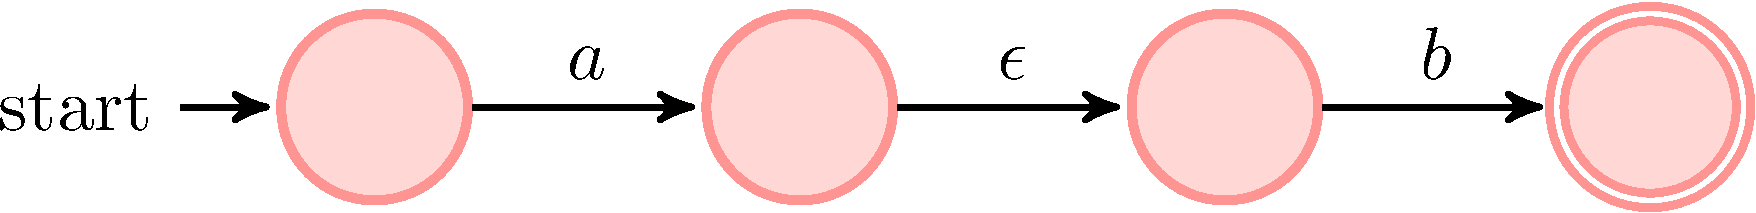
\includegraphics[scale=0.22]{ab.pdf}\end{centering}
		\item[]
		\item[{\color{green}\texttt{a*}}]
\begin{centering}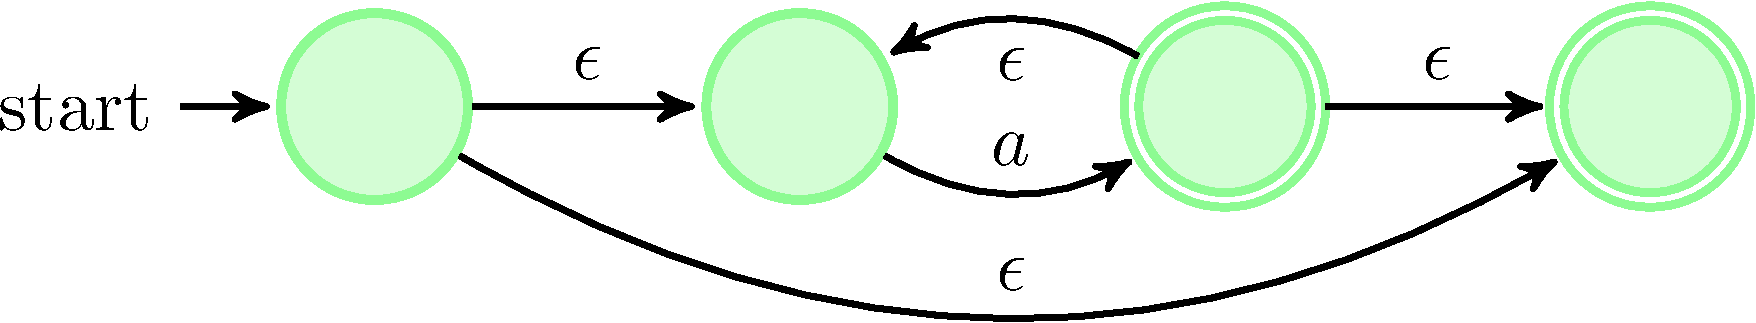
\includegraphics[scale=0.22]{astar.pdf}\end{centering}
		\item[]
		\item[{\color{blue}\texttt{(a|b)}}]
\begin{centering}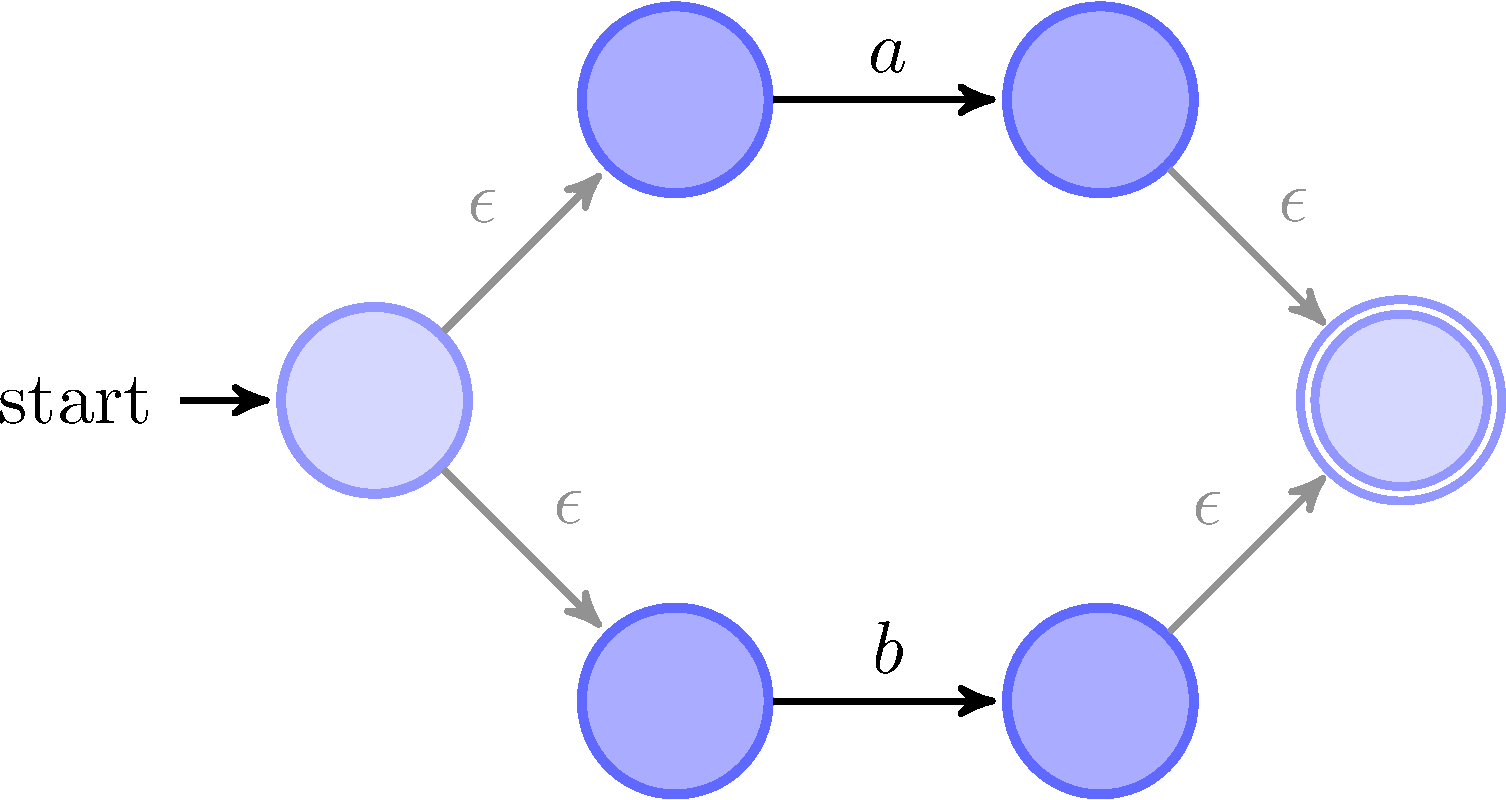
\includegraphics[scale=0.22]{aorb.pdf}\end{centering}
	\end{itemize}
\end{frame}

\begin{frame}[plain]
    \frametitle{Thompson's Algorithmus: Beispiel}
	\begin{itemize}
		\item[] Regulärer Ausdruck: \texttt{a(a|b)c*}
		\item[]
		\item[]
	\end{itemize}
	\begin{centering}
		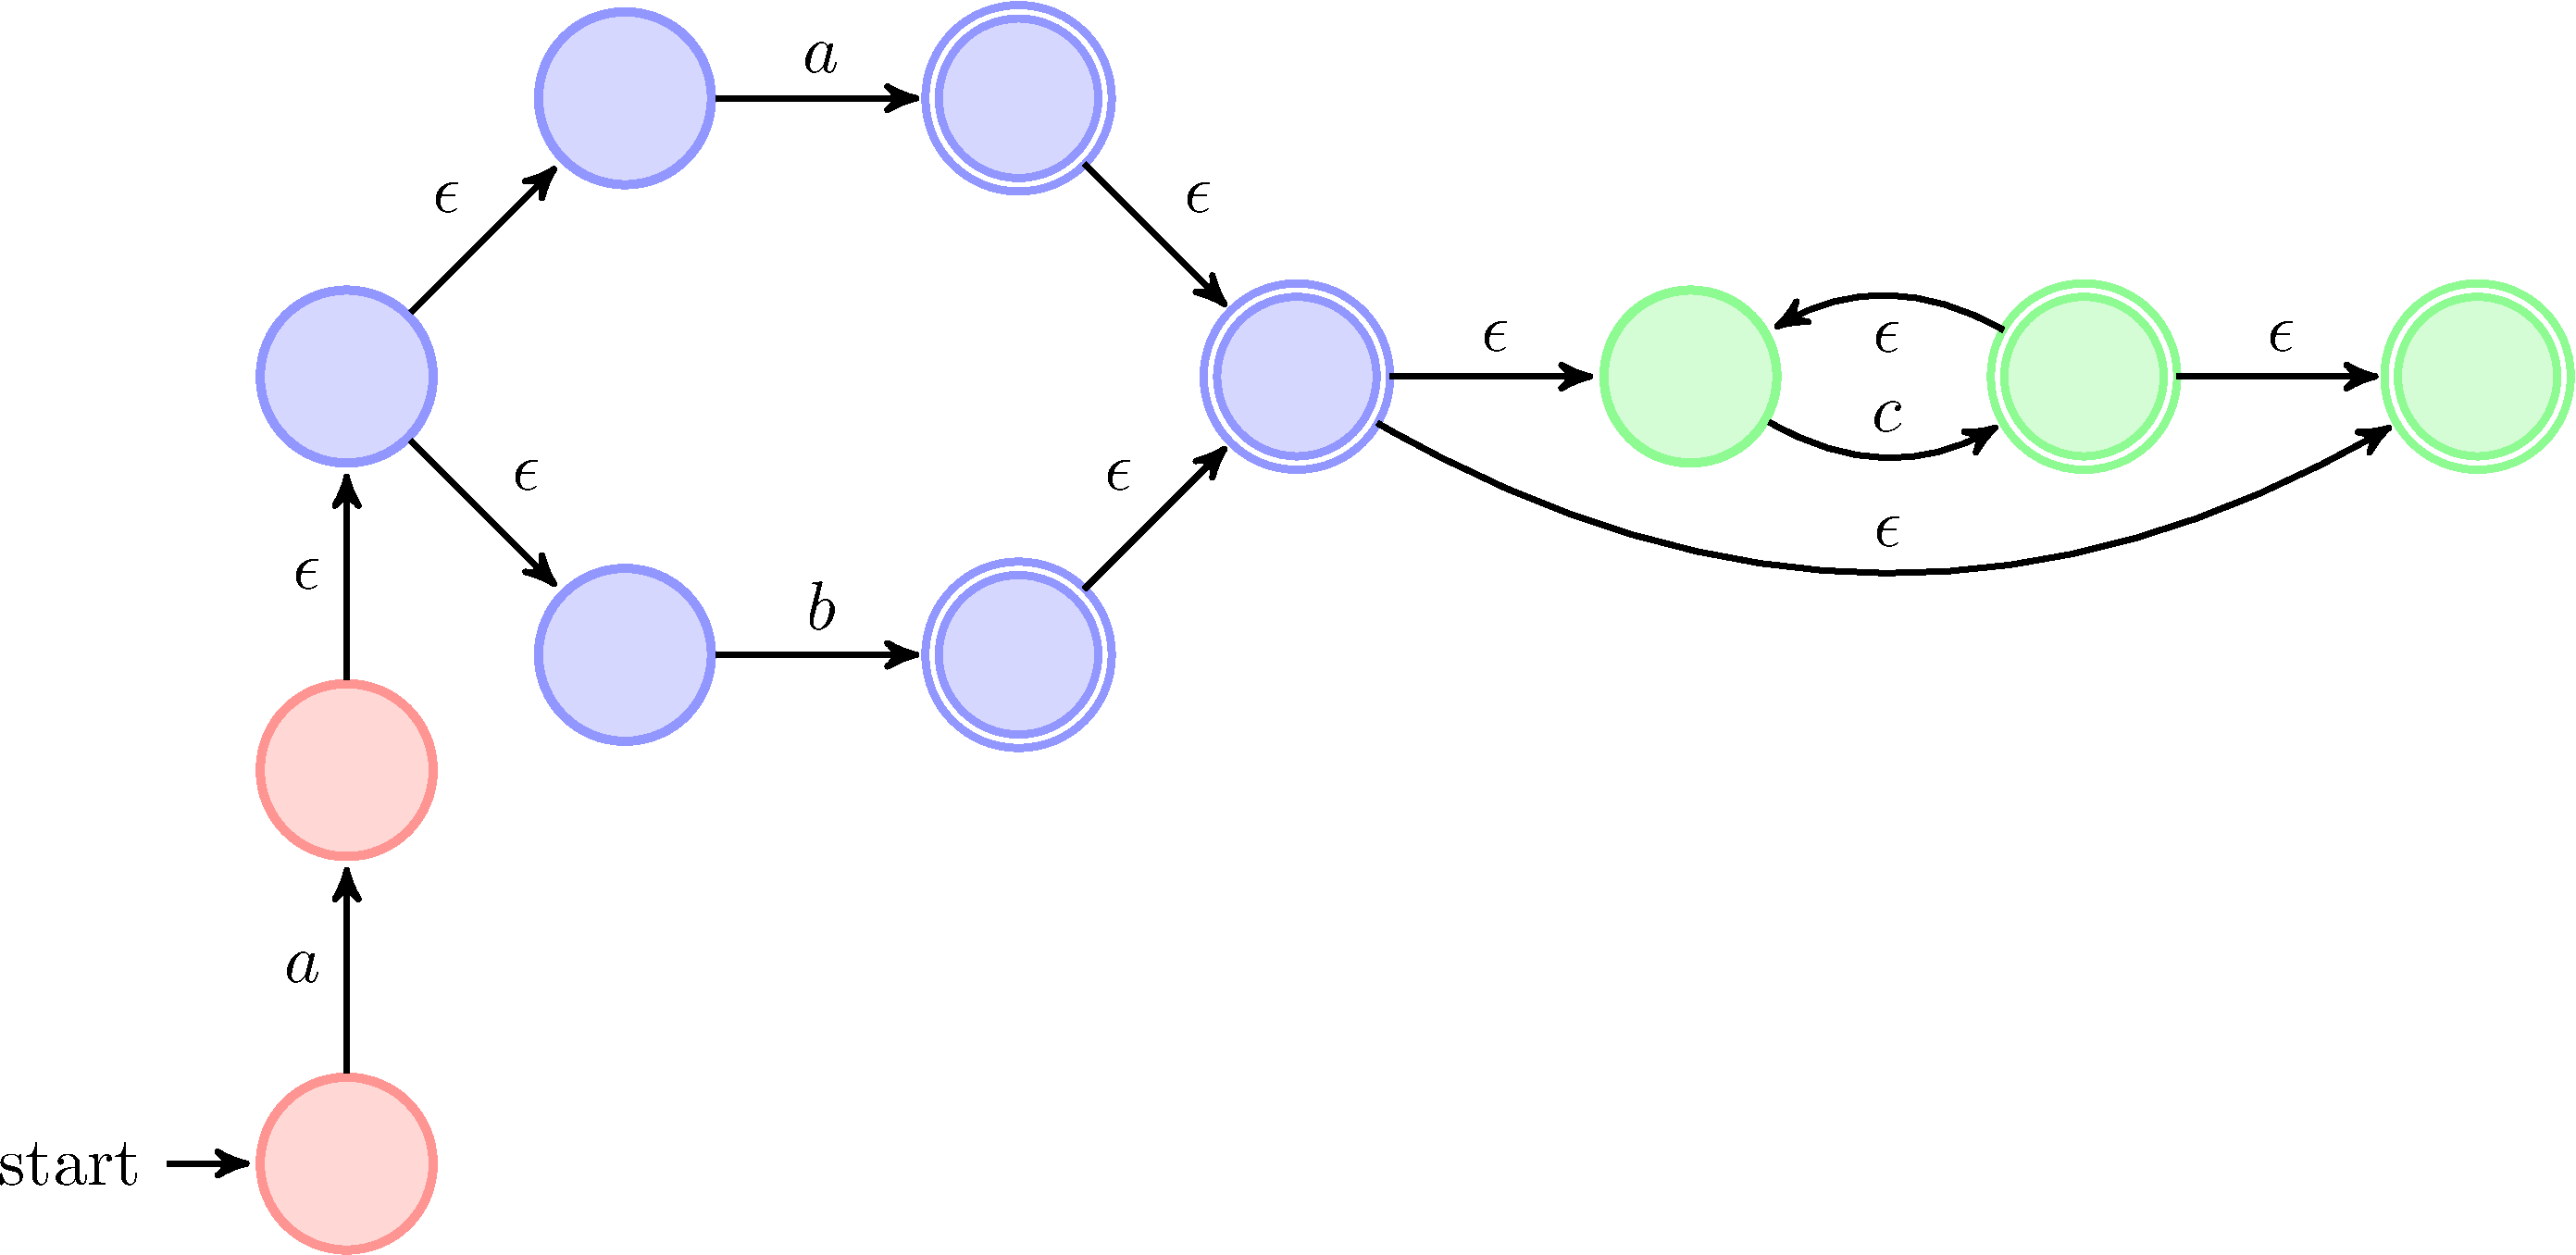
\includegraphics[scale=0.23]{aabc.pdf}
	\end{centering}
\end{frame}


\subsection{Recursive Descent Methode}
\begin{frame}
    \frametitle{Recursive Descent Methode}

\end{frame}
%%%%%%%%%%%%%%%%%%%%%%%%%%%%%%%%%%%%%%%%%%%%%%%%%%%%%%%%%%%%%%%%%%%%%%%%%%%%%%





%%%%%%%%%%%%%%%%%%%%%%%%%%%%%%%%%%%%%%%%%%%%%%%%%%%%%%%%%%%%%%%%%%%%%%%%%%%%%%
\begin{frame}[allowframebreaks]
    \frametitle{Literatur}
    \bibliographystyle{alpha}
    \bibliography{beamer}
    \nocite{*}
\end{frame}
%%%%%%%%%%%%%%%%%%%%%%%%%%%%%%%%%%%%%%%%%%%%%%%%%%%%%%%%%%%%%%%%%%%%%%%%%%%%%%


\begin{frame}[plain]
\end{frame}


\end{document}

